\section{Nota teórica}
En esta sección del laboratorio, se exponen los principales componentes que usarán para el proyecto a realizar: un voltímetro.
\subsection*{Arduino UNO}
Se usará la placa de Arduino UNO que posee el microcontrolador ATMega382P.

\subsubsection*{Características generales}
Sus detalles se describen a continuación:
\begin{itemize}
\item Es un MCU de 8 bits.
\item Posee arquitectura RISC/Harvard.
\item 4/8/16/64 kb memoria flash.
\item 512b/1/2kb de memoria SRAM.
\item 1/2kb de EEPROM.
\item 23 GPIOS.
\item Timer/Counters de 8 y 16 bits.
\item Posee interrupciones.
\item 8 canaels PWM y comparador analógico.
\item 6 canales 10-bit ADC.
\item Posee protocolo SPI y USART (Universal Synchronous/Asynchronous Receiver/Transmitter) I2C.
\end{itemize}
\subsubsection*{Diagrama de bloques y pines}
El diagrama de bloques de este MCU se muestra en la figura \ref{fig1}.

\begin{figure}[H]
\centering
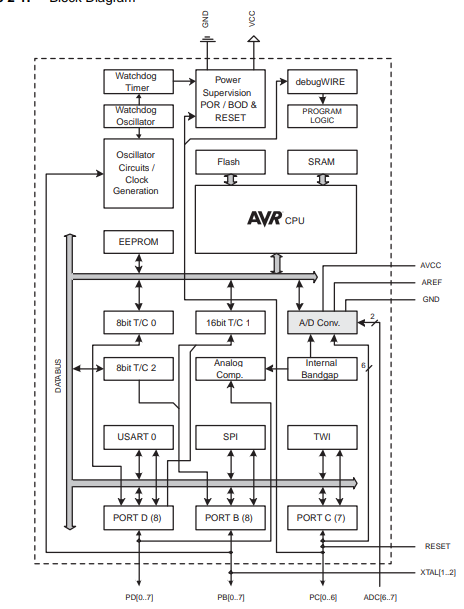
\includegraphics[width=.8\linewidth]{Imagenes/1.png}
 \caption{Diagrama de bloques de ATMega328P. Tomado de \cite{web}.}
 \label{fig1}
\end{figure}

\begin{figure}[H]
\centering
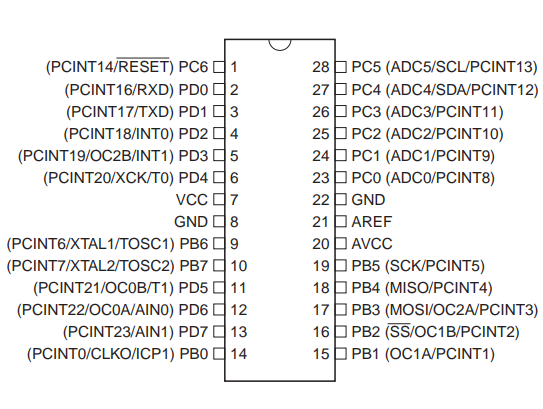
\includegraphics[width=.8\linewidth]{Imagenes/2.png}
 \caption{Diagrama de pines de ATMega328P. Tomado de \cite{web}.}
 \label{fig2}
\end{figure}
\subsubsection*{Características eléctricas}
La siguiente lista describe estos detalles.
\begin{itemize}
\item Voltaje: 1.8-\SI{5.5}{\volt}.
\item Velocidad: 0-\SI{4}{\mega\Hz},  1.8-\SI{5.5}{\volt}. 0-\SI{10}{\mega\Hz},  2.7-\SI{5.5}{\volt}. 0-\SI{20}{\mega\Hz},  4.5-\SI{5.5}{\volt}
\item Modo activo: \SI{0.3}{\mA}
\item Temperatura de funcionamiento: $-55^\circ$ a +$125^\circ$.
\item Temperatura de almacenamiento: $-65^\circ$ a +$125^\circ$.
\item Temperatura pin RESET y GND: -\SI{0.5}{\volt} a \SI{13}{\volt}.
\item Temperatura en los demás pines: -\SI{0.5}{\volt} a VCC\SI{0.5}{\volt}.
\item Corriente por pin I/O: \SI{40}{\mA}.


\end{itemize}

\subsection*{Periféricos utilizados}

\subsection*{Componentes electrónicos complementarios}

    
\subsection*{Lista de componentes}

\begin{table}[H]
\caption{Lista de equipos}
\label{table_2}
\begin{center}
\begin{tabular}{r|cc}
\hline
\textbf{Componente}&\textbf{Cantidad}&\textbf{Precio}\\
 \hline
Arduino UNO&1   &-- \\ \hline 
Resistencias &1   &-- \\ \hline 
Capacitancias&1   &-- \\ \hline 
LEDs&1   &-- \\ \hline 
Pantalla PCD8544&1   &-- \\ \hline 
Botón&1   &-- \\ \hline 
 \textbf{Total}& &  \\
 \hline
\end{tabular}
\end{center}
\end{table}

\subsection*{Diseño del circuito}
\newpage
